\documentclass[landscape,a4paper,8pt]{scrartcl}

\usepackage{bm}
\usepackage{layout}
\usepackage{changepage}   % for the adjustwidth environment
\usepackage{booktabs}
%\usepackage{extsizes}
%\usepackage[all=normal,paragraphs=normal,mathdisplays=tight]{savetrees}
\usepackage{xargs} 
\usepackage{graphicx,xcolor} 
\usepackage[bordercolor=white,backgroundcolor=gray!30,linecolor=black,colorinlistoftodos]{todonotes}
\newcommandx{\tim}[1]{\todo[color=blue!30, inline]{tim: {#1}}}

%------------------------------------
%  FOOTER SETTINGS
%------------------------------------
\pagestyle{fancy}
\renewcommand{\headrulewidth}{0pt}
\fancyhead{}
\renewcommand{\footrulewidth}{0.5pt}
\fancyfoot[L]{\footnotesize\color{dkgreen} Tim Taubner, Jen Wei Niam; \href{https://github.com/timethy/mpc}{www.github.com/timethy/mpc}}
\fancyfoot[C]{\footnotesize\color{dkgreen} Model Predictive Control -- \today}
\fancyfoot[RO, LE] {\footnotesize\color{dkgreen} \thepage}

\renewcommand{\iff}{\Leftrightarrow}
\renewcommand{\implies}{\Rightarrow}
\newcommand{\remph}[1]{{\textcolor{red}{#1}}}
\newcommand{\mc}[1]{\mathcal{#1}}
\newcommand{\R}{\mathbb R}
\newcommand\va{\bm{a}}
\newcommand\vb{\bm{b}}
\newcommand\vq{\bm{q}}
\newcommand\vr{\bm{r}}
\newcommand\vp{\bm{p}}
\newcommand\vk{\bm{k}}
\newcommand\vn{\bm{n}}
\newcommand\vv{\bm{v}}
\newcommand\vx{\bm{x}}
\newcommand\vy{\bm{y}}
\newcommand\vz{\bm{z}}
\newcommand\vA{\bm{A}}
\newcommand\vB{\bm{B}}
\newcommand\vC{\bm{C}}
\newcommand\vD{\bm{D}}
\newcommand\vE{\bm{E}}
\newcommand\vF{\bm{F}}
\newcommand\vG{\bm{G}}
\newcommand\vH{\bm{H}}
\newcommand\vI{\bm{I}}
\newcommand\vK{\bm{K}}
\newcommand\vL{\bm{L}}
\newcommand\vM{\bm{M}}
\newcommand\vN{\bm{N}}
\newcommand\vO{\bm{O}}
\newcommand\vP{\bm{P}}
\newcommand\vQ{\bm{Q}}
\newcommand\vR{\bm{R}}
\newcommand\vS{\bm{S}}
\newcommand\vT{\bm{T}}
\newcommand\vU{\bm{U}}
\newcommand\vV{\bm{V}}
\newcommand\vW{\bm{W}}
\newcommand\vX{\bm{X}}
\newcommand\vY{\bm{Y}}
\newcommand\vZ{\bm{Z}}

\newcommand{\Mn}[1]{\begin{pmatrix}#1\end{pmatrix}} %normale Klammern, normal bracket
\newcommand{\Mo}[1]{\begin{matrix}#1\end{matrix}} %ohne Klammern, no brackets
\newcommand{\Me}[1]{\begin{bmatrix}#1\end{bmatrix}} %eckige Klammern
\newcommand{\Mg}[1]{\begin{Bmatrix}#1\end{Bmatrix}} %geschweifte Klammern

\DeclareMathOperator\argmin{argmin}
\DeclareMathOperator\argmax{argmax}
\DeclareMathOperator\diag{diag}
\DeclareMathOperator\pre{pre}
\DeclareMathOperator\norm{norm}
\DeclareMathOperator\rank{rank}
\DeclareMathOperator\dom{dom}
\DeclareMathOperator\size{size}

%------------------------------------
%  BEGIN DOCUMENT
%------------------------------------

\begin{document}
\raggedright
%\sffamily

%--CONTENT--
\begin{multicols*}{3}
\section{System Theory}
\subsection{Nonlinear Systems}
\begin{align*}
\dot x    & = g(x, u)         & y   & = h(x, u) \\
\dot{x_s} & = g(x_s, u_s) = 0 & y_s & = h(x_s, u_s) \\
\vA^c     & = \frac{\partial g}{\partial x^T}\bigg\rvert_{x=x_s, u=u_s} & \vB^c & = \frac{\partial g}{\partial u^T}\bigg\rvert_{x=x_s, u=u_s} \\
\vC^c     & = \frac{\partial h}{\partial x^T}\bigg\rvert_{x=x_s, u=u_s} & \vD^c & = \frac{\partial h}{\partial u^T}\bigg\rvert_{x=x_s, u=u_s}
\end{align*}

\subsection{Linear Systems}
\paragraph{Continuous}
\begin{align*}
\dot{x}(t) &= \vA^cx(t)+\vB^cu(t)\\
x(t) &= e^{\vA^c(t-t_0)}x_0+\int_{t_0}^te^{\vA^c(t-\tau)}\vB u(\tau)d\tau \\
e^{\vA^ct}&=\sum_{n=0}^\infty\frac{(\vA^ct)^n}{n!}
\end{align*}
\paragraph{Discrete}
\begin{align*}
x_{k+1} &= \vA x_k+\vB u_k\\
y_k &= \vC x_k + \vD u_k\\
x_{k+N}&=\vA^N x_k+\sum_{i=0}^{N-1}\vA^i\vB u_{k+N-1-i}
\end{align*}

\subparagraph{Forward Euler} $A = I + T_s A^c ,\ B = T_s B^c ,\ C = C^c ,\ D = D^c $
\begin{align*}
x_{k + 1} &= x_k + T_s g^c(x_k,u_k) = g(x_k,u_k) \\
y_{k}     &= h^c(x_k, u_k) = h(x_k, u_k)
\end{align*}

\subparagraph{Exact discretization} (assume constant $u(t)$ during $T_s$)
\begin{align*}
\vA & = e^{\vA^cT_s},\ \vB = \int_0^{T_s} e^{\vA^c(Ts-\tau')}\vB^cd\tau \\
\vB & = (\vA^c)^{-1}(\vA-\vI)\vB^c,\ \text{if $\vA^c$ invertible}
\end{align*}

\subsection{Lyapunov Stability}
System is stable in the sense of Lyapunov iff it stays in any arbitrarily small neighborhood of the origin when it is disturbed slightly.
\paragraph{Lyapunov stable} iff $\forall\epsilon > 0 \; \exists\delta(\epsilon)$ s.t.\
$\lVert x_0 \rVert < \delta(\epsilon)\to \lVert x_k \rVert < \epsilon, \forall k \geq 0$
\paragraph{asymptotically stable} in $\Omega\subseteq \R^n$ if Lyapunov stable and \emph{attractive} $\lim_{k\to\infty}x_k=0, \forall x_0\in \Omega$.

\paragraph{Lyapunov Function $V: \R^n \to \R$}
continous at the origin, finite $\forall x \in \Omega$,
\begin{align*}
V(0) = 0 \text{ and } V(x)>0, \forall x\in \Omega \backslash \{0\}\\
V(g(x))-V(x) \leq -\alpha(x), \forall x\in\Omega\backslash \{0\}
\end{align*}
where $\alpha: \R^n\to\R$ is continuous positive definite, equilibrium at $x=0$
and $\Omega\subset\R^n$ closed and bounded set containing the origin.

\paragraph{Lyapunov Theorem}
If system admits Lyapunov function $V(x)$, then $x=0$ is \remph{asymptotically stable} in $\Omega$ (sufficient but not necessary).

If additionally $\lVert x \rVert \to \infty \implies V(x) \to \infty$ \remph{globally asymptotically stable}.

To check if $V(x) = x^T\vP x$ is valid Lyapunov function of system $x_{k+1} = \vA x_k$ check if $(\vA\vP\vA-\vP)$ has neg.\ eigen values.

In other words: Iff eigenvalues of $A$ inside unit circle (i.e. stable) then $\exists unique \ \vP>0$ that solves $\vA_{cl}^T\vP\vA_{cl}-\vP = -\vQ,\ \vQ > 0$ and $V(x) = x^T\vP x$ is a lyapunov function.

\subsection{Observability $\implies$ Detectability, Controllability $\implies$ Stabilizability}
\paragraph{$(A,C)$ observable}
if $\rank(\vO) = n$ (full col. rank) for
$\vO = \Me{C^T \\ (CA)^T \\ \dots \\ (CA^{n-1})^T}$ or $\rank\Me{\vA-\lambda\vI \\ \vC} = n \; \remph{\forall} \lambda_i$ of $\vA$ (PBH-test).
\paragraph{$(A,C)$ detectable}
iff $\rank\Me{\vA-\lambda\vI \\ \vC} = n \remph{\forall \text{unstable}} |\lambda_i| \geq 1$ of $\vA$.

\paragraph{$(A,B)$ controllable}
if $\rank\vC = n$,
$\vC = \Me{\vB & \vA\vB & \dots & \vA^{n-1}\vB}$
or
if $\rank\left(\Me{\lambda_j \vI - \vA & \vB}\right) = n\; \remph{\forall} \lambda_i$ of $\vA$ (PBH-test).

Intuition: Can reach any state in (at most) $n$ steps.

\paragraph{$(A,B)$ stabilizable}
if $\rank\Me{\lambda_j \vI - \vA & \vB} = n \; \remph{\forall \text{unstable}} |\lambda_i| \geq 1$ of $\vA$.

Intuition: Can reach origin in (at most) $n$ steps.

\section{Unconstrained Control}
\subsection{Block Approach (used also for $\bar w$ substition)}
\begin{align*}
		\Me{x_0 \\ x_1 \\ \vdots \\ x_N } & = \Me{\vI \\ \vA \\ \vdots \\ \vA^N}x(0) + \Me{\bm 0 & \bm 0 & \dots & \bm 0 \\ \vB & \bm 0 & \dots & \bm 0 \\ \vA\vB & \vB & \dots & \bm 0 \\ \vdots & \vdots & \ddots & \bm 0 \\ \vA^{N-1}\vB & \dots & \vA\vB & \vB}\Me{u_0 \\ u_1 \\ \vdots \\ u_{N_1}}
\end{align*}

\begin{align*}
x & = \vS^x\cdot x(0) + \vS^u\cdot u & \size(\vS^x) & = \left[ n_\text{states} \cdot (N+1) , N \right] \\
  &                                  & \size(\vS^u) & = \left[ n_\text{states} \cdot (N+1), n_\text{states} \right] \\
\bar\vQ & = \diag(\vQ,\dots,\vQ, \vP) & \size(\bar\vQ) & = \left[ n_\text{states} \cdot (N+1), n_\text{states} \cdot (N+1) \right] \\
\bar\vR & = \diag(\vR,\dots,\vR) & \size(\bar\vR) & = \left[ n_\text{input}\cdot N, n_\text{input}\cdot N \right] \\
\vH & = {\vS^u}^T\bar\vQ\vS^u + \vR & \vF & = {\vS^x}^T\bar\vQ\vS^u \\
\vY & = {\vS^x}^T\bar\vQ\vS^x
\end{align*}
\paragraph{Optimal cost and control}
%\quad \nabla_{u_0}J^*(x_0) \mbeq 0 \text{ gives} \\
\begin{align*}
J^*(x_0) & = -x_0^T \vF\vH\vF^T x_0 + x_0^T \vY x_0 \\
u^*(x_0) & = -\vH^{-1}\vF^T x_0 = - \left( {\vS^u}^T\bar\vQ\vS^u + \vR \right)^{-1}{\vS^u}^T\bar\vQ\vS^x x_0 \\
\end{align*}

\subsection{Recursive Approach}
\begin{align*}
J_k^*(x_k) & = \min_{u_k} I(x_k, u_k) + J_{k+1}(x_{k+1})
\end{align*}
Is a feedback controller as opposed to the Batch Approach.
For LQR solve via Riccati Difference Equation (RDE).
\begin{align*}
 \vF_k & = -(\vB^T\vP_\remph{k+1}\vB + \vR)^{-1}\vB^T\vP_\remph{k+1}\vA \\
 \vP_k & = \vA^T\vP_\remph{k+1}\vA + \vQ - \vA^T\vP_\remph{k+1}\vB(\vB^T\vP_\remph{k+1}\vB + \vR)^{-1}\vB^T\vP_\remph{k+1}\vA
\end{align*}
\begin{align*}
 u_k^* & = \vF_k\ x_k  & J_k^*(x_k) & = x_k^T\vP_k\ x_k & \vP_N & = \vP
\end{align*}
For unconstrained Infinite Horizon Problem, substituting $\vP_\infty = \vP_k = \vP_{k+1}$ into RDE gives DARE.
Uniquely solvable, iff $(A,B)$ stabilizable and $(A, G)$ detectable, where $\vG\vG^T = \vQ$.
Follows from closed-loop system $x_{k+1} = (\vA + \vB\vF_k)x_k$

\section{(Convex) Optimization}

\paragraph{General Problem}
$\min_{x \in \dom(f)} f(x)$ s.\ t.\ $g_i(x) \leq 0$ and $h_j(x) = 0.$
%for $i = 1,\dots,m, j = 1,\dots,p$.

\paragraph{Norm $f(x): \R^n \rightarrow \R$}
\begin{align*}
f(x) & = 0 \implies x = 0, && f(x) \geq 0 \\
f(\alpha \cdot x) & = |\alpha|\cdot f(x) && \text{for scalar } \alpha \\
f(x+y) & \leq f(x) + f(y) && \forall x, y \in R^n
\end{align*}

\subsection{Convexity}
\paragraph{Convex set $\mc X$} iff $\forall \lambda \in [0, 1] \forall x, y \in \mc X\ \lambda x + (1-\lambda) y \in \mc X$.
Intersection preserves convexity, union does not.
\paragraph{Affine set $\mc X$} $= \{ x \in \R^n | \vA x = b \}$ for some $\vA,b$
\paragraph{Subspace} is affine set through origin, i.e. $b = \bm 0$, aka Nullspace of $\vA$.
\paragraph{Hyperplane $\mc X$} $= \{ x \in \R^n | a^T x = b \}$ for some $a, b$.
\paragraph{Halfspace $\mc X$} $= \{ x \in \R^n | a^T x \leq b \}$ for some $a, b$.
\paragraph{Polyhedron $\mc P$} $= \{ x | a_i^Tx \leq b_i, i = 1, \dots, n \} = \{ x | \vA x \leq b \}$
\paragraph{Cone $\mc X$} if for all $ x \in \mc X $, and for all $\theta > 0, \theta x \in \mc X$.
\paragraph{Ellipsoid $\mc E$} $= \{ x | (x-x_c)^T\vA^{-1}(x-x_c) \leq 1 \}$, $x_c$ center point.
\paragraph{Convex function $f : \text{dom($f$)} \rightarrow \R$} is convex iff dom($f$) is convex and
$f (\lambda x + (1 - \lambda)y) \geq \lambda f(x) + (1-\lambda)f(y), \forall \lambda \in (0, 1), \forall x, y \in \text{dom($f$)}$.
\paragraph{Norm ball} is convex (for all norms).
\paragraph{Epigraph set $f : \text{dom($f$)} \rightarrow \R$} is the set $\text{epi($f$)} :=
\left\{ \Me{x\\t} | x \in \text{dom($f$)}, f(x) \le t \right\} \subseteq \text{dom($f$)} \times \R$
\paragraph{Level set $L_a$} of a function $f$ for value $a$ is the set of all $x \in \text{dom($f$)}$ for which $f(x) = a$: $L_a = \left\{x | x \in \text{dom($f$)}, f(x) = a\right\}$.
\paragraph{Sublevel set $C_a$} is defined by $C_a = \left\{x | x \in \text{dom($f$)}, f(x) \le a\right\}$.


\subsection{Linear Programming (LP)}
\paragraph{Problem statement} $\min c^Tx$ such that $\vG x \leq h$ and $\vA x = b$.
\paragraph{Norm $l_\infty$}
$\min_x \lVert x \rVert_\infty = \min_{x \in \R^n} \left[ \max\{x,\dots,x_n,-x_1,\dots,-x_n\}\right]$:
\begin{align*}
     & \min_{x,t} t & \text{subject to}\quad & x_i \leq t, -x_i \leq t,   \; & \vF x \leq g \\
\iff & \min_{x,t} t & \text{subject to}\quad & -{\bm 1} t \leq x \leq {\bm 1} t,\; & \vF_x \leq g.
\end{align*}

\paragraph{Norm $l_1$}
$\min_x \lVert x \rVert_1 = \min_x\left[\sum_{i=1}^{m} \max\{x_i,-x_i\}\right]$:
\begin{align*}
     & \min_{t} t_1 + \dots + t_m & \text{subject to}\quad & x_i \leq t_i, -x_i \leq t_i,\; & \vF x \leq g \\
\iff & \min_{t} {\bm 1}^Tt    & \text{subject to}\quad & -t \leq x \leq t,\;            & \vF_x \leq g.
\end{align*}
Note that for $\dim x = 1$, $l_1$ and $l_\infty$ are the same.
Note also that $t$ is scalar for norm $l_\infty$ and a vector in norm $l_1$.

\paragraph{Piecewise Affine}
\begin{align*}
\min_x \left[ \max_{i=1,\dots,m} \{ c_i^Tx + d_i \} \right] & \quad \text{s.t.\ } \vG x \leq h \\
\iff \min_{x,t} t & \quad \text{s.t.\ } c_i^T x + d_i \leq t, \vG x \leq h
\end{align*}

\subsection{Duality}
\paragraph{Lagrangian Dual Function}
\begin{align*}
	L(x,\lambda,\nu) & = f(x) + \sum_{i=1}^{m}\lambda_i g_i(x) + \sum_{i=1}^{p}\nu_i h_i(x) \\
	d(\lambda,\nu) & = \inf_{x \in \mc{X}} L(x,\lambda,\nu) \quad \text{ i.e. } \nabla_x L(x, \lambda, \nu) = 0
%	&= \inf_{x \in \mc{X}} \left[ f_0(x)+\sum_{i=1}^{m}\lambda_i f_i(x)+\sum_{i=1}^{p}\nu_i h_i(x)\right]
\end{align*}
\paragraph{Dual Problem (always convex)} 
$\max_{\lambda,\nu} d(\lambda,\nu)$ s.\ t.\ $\lambda \geq 0$. \\
Optimal value is lower bound for primal: $d^* \leq p^*$.

If primal convex, \remph{Slater condition} (strict feasibility) implies \emph{strong duality}:
$\left\{x \left| \right. Ax=b, f_i(x)<0, \right\} \neq \emptyset \Rightarrow d^*  = p^* $
%
\paragraph{Karush-Kuhn-Tucker (KKT) Conditions}
are necessary for optimality (and sufficient if primal convex).
\begin{align*}
& \text{Primal Feasability} & f_i(x^*)  &\leq 0 \quad && i=1,\dots,m \\
&                           & h_i(x^*)  &=0 \quad && i=1,\dots,p \\
& \text{Dual Feasability}        & \lambda^* & \geq 0 && \\
& \text{Complementary slackness} & \lambda_i^* \cdot f_i(x^*) & = 0 && i = 1,\dots,m \\
& \text{Stationarity} & \nabla_x L(x^*,\lambda^*,\nu^*) & = 0 && \\
%&\nabla f_0(x^*) + \sum_{i=1}^m\lambda_i^*\nabla f_i(x^*)+  \sum_{i=1}^p\nu_i^*\nabla h_i(x^*)
\end{align*}
%
\paragraph{Dual of LP}
\begin{align*}
     \min_x c^T x & \quad \text{s.t.\ } \vA x = b, \vC x \leq e \\
\iff \max_{\lambda,\nu} -b^T\nu - e^T\lambda & \quad \text{s.t.\ } A^T\nu + C^T\lambda + c = 0, \lambda \geq 0
\end{align*}

\paragraph{Dual of QP}
\begin{align*}
     & \min_x \frac{1}{2}x^T\vQ x + c^T x \quad \text{s.t.\ } \vC x \leq e \\
\iff & \min_{\lambda,\nu} \frac{1}{2}\lambda^T\vC\vQ^{-1}\vC^T\lambda + (\vC\vQ^{-1}c + e)^T\lambda + \frac{1}{2} c^T \vQ^{-1}c \\
     & \text{s.t.\ } \vQ x + \nu + c^T \lambda = 0, \lambda \geq 0
\end{align*}

\section{Constrained Finite Time Optimal Control (CFTOC)}
\subsection{MPC with linear cost}
\begin{align*}
J(x_0, u) = \lVert \vP x_N \rVert_p + \sum_{i=0}^{N-1} \lVert \vQ x_i \rVert_p + \lVert \vR u_i \rVert_p.
\end{align*}
The CFTOC problem can be formulated as an $\infty$-norm LP problem as shown below.
\begin{align*}
\min_z\ & \epsilon_0^x + \dots + \epsilon_N^x + \epsilon_0^u + \dots + \epsilon_{N-1}^u \\
\text{s.t. } & -\bm{1}_n\epsilon_i^x \leq \pm \vQ \left[\vA^i x_0 + \sum_{j=0}^{i-1}\vA^j\vB u_{i-1-j}\right] \\
             & -\bm{1}_r\epsilon_N^x \leq \pm \vP \left[\vA^N x_0 + \sum_{j=0}^{N-1}\vA^j\vB u_{N-1-j}\right] \\
             & -\bm{1}_m\epsilon_N^u \leq \pm \vR u_i \\
						 & x_i = \vA^i x_0 + \sum_{j=0}^{i-1}\vA^j\vB u_{i-1-j} \in \mc X \\
						 & x_N = \vA^Nx_0 + \sum_{j=1}^{N-1}\vA^j\vB u_{N-1-j} \in \mc X \\
						 & u_i \in \mc U
\end{align*}
Converting to LP form:
\begin{align*}
&\min_z\ c^Tz \quad \\ \text{s.t. } &\bar \vG z \leq \bar w + \bar s x_k \\
    z = & \Me{\epsilon_0^x & \dots & \epsilon_N^x & \epsilon_0^u & \dots & \epsilon_{N-1}^u &u_0^T &\dots &u_{N-1}^T} \\
    c = & \Me{1 & \dots & 1 & 1 & \dots & 1 & 0 & \dots & 0} \\
\bar\vG = & \Me{\vG_\epsilon & \bm{G}_u \\ 0 & \bm{G}}, \quad \bar w = \Me{w_\epsilon \\ w}, \quad \bar s = \Me{s_\epsilon \\ s} 
\end{align*}
Where $\bm{G}$ is the normal problem constraints and $[\vG_\epsilon \bm{G}_u]$ form the constraints of the newly introduced variable $\epsilon$ as given in the first 3 constraints in the section above. For example, we require:
\begin{gather*}
	-\epsilon_i^u \le u_i \le \epsilon_i^u \\
	-\epsilon_0^x \le Ax_0 + Bu_0 \le \epsilon_0^x \\
	-\epsilon_1^x \le A^2x_0 + Bu_1 + ABu_0 \le \epsilon_1^x
\end{gather*}

\subsection{QP with substitution (see also Batch approach)}
\begin{align*}
J^*(x_k) & = \min_u \Me{u^T & x_k^T}\Me{\vH & \vF^T \\ \vF & \vY}\Me{u \\ x_k} \\
\text{s. t. } & \vG\ u \leq w + \vE\ x_k
\end{align*}
Latter gives three sets (same for without substitution)
\begin{align*}
\mc{X}   & = \{ x | A_x\ x \leq b_x\} \\
\mc{U}   & = \{ u | A_u\ u \leq b_u\} \\
\mc X_f & = \{ x | A_f\ x \leq b_f\}
\end{align*}
State equations are in cost matrix, usually in the form: $\vA_x = \Me{1 \\ -1}, b_x = \Me{b_\text{max} \\ -b_\text{min}}$
\begin{scriptsize}
\setlength{\arraycolsep}{2pt}
\begin{align*}
\vG & = \Me{\vA_u & 0 & \dots & 0 \\
          0 & \vA_u & \dots & 0 \\
          \vdots & \vdots & \ddots & \vdots \\
					0      & 0 & \dots & \vA_u \\
					0      & 0 & \dots & 0 \\
					\vA_x\vB & 0 & \dots & 0 \\
					\vA_x\vA\vB & \vA_x\vB & \dots & 0 \\
					\vdots & \vdots & \ddots & \vdots \\
					\vA_x\vA^{N-2}\vB & \vA_x\vA^{N-3}\vB & \dots & 0 \\
					\vA_f\vA^{N-1}\vB & \vA_f\vA^{N-2}\vB & \dots & \vA_f\vB} &
\vE & = \Me{0 \\ 0 \\ \vdots \\ 0 \\ -\vA_x \\ -\vA_x\vA \\ -\vA_x\vA^2 \\ \vdots \\ -\vA_x\vA^{N-1} \\ -\vA_f\vA^N} &
\vW & = \Me{b_u \\ b_u \\ \vdots \\ b_u \\ b_x \\ b_x \\ b_x \\ \vdots \\ b_x \\ b_f}
\end{align*}
\end{scriptsize}

\subsection{QP without substitution}
State equations represented in equality constraints ($k$ fixed, usually $k=0$).
\begin{align*}
J^*(x_k) = \min_z\ & \Me{z^T & x_k^T}\Me{\bar\vH & \bm 0 \\ \bm 0 & \vQ}\Me{z \\ x_k} \\
\text{s.t.}      \ & \vG\ z \leq w + \vE\ x_k \\
                   & \vG_\text{eq}\ z = \vE_\text{eq}\ x_k, \quad \text{system dynamics}
\end{align*}
$\bar\vH = \diag(\vQ,\dots,\vQ,\vP,\vR,\dots,\vR)$
\begin{scriptsize}
\setlength{\arraycolsep}{2pt}
\begin{align*}
z & = \Me{x_1 \\ . \\ x_N \\ u_0 \\ . \\ u_{N-1}} &
\vG_\text{eq} & =
\begin{bmatrix}[rrrr@{\hskip 2pt}|@{\hskip 2pt}rrrr]
 \vI & \   &  \   & \   & -\vB &  \   & \ &  \ \\
-\vA & \vI &  \   & \   &  \   & -\vB & \ &  \ \\
 \   & .   & .    & \   &  \   &  \   & . &  \ \\
 \   & \   & -\vA & \vI &  \   &  \   & \ & -\vB
\end{bmatrix} &
\vE_\text{eq} & = \Me{\vA \\ 0 \\ . \\ 0} \\
w & = \Me{b_x \\ . \\ b_f \\ b_u \\ . \\ b_u} &
\vG & =
\begin{bmatrix}[cccc|ccc]
 0  & \     & \ & \     & \     & \ & \ \\
 \  & \vA_x & \ & \     & \     & \ & \ \\
 \  & \     & . & \     & \     & \ & \ \\
 \  & \     & \ & \vA_x & \     & \ & \ \\ \cmidrule(lr){1-7}
 \  & \     & \ & \     & \vA_d & \ & \ \\
 \  & \     & \ & \     & \     & . & \ \\
 \  & \     & \ & \     & \     &   & \vA_d
\end{bmatrix} &
\vE & = \Me{-\vA_x^T \\ 0 \\ . \\ 0}
\end{align*}
\end{scriptsize}

\subsection{Invariance}
\paragraph{Pos.\ Invariant set $O$} iff $x_k \in O \implies x_{k+1} = g(x_k) \in O \; \forall k$.
\paragraph{Max.\ Pos.\ Invariant set $O_\infty \subset \mc X$} iff $0 \in O_\infty$, $O_\infty$ invariant and contains all invariant sets $O$ with $0 \in O$.
\paragraph{Pre-Set $\pre(S)$}
$:= \{ x | g(x) \in S\} = \{ x | \vA x \in S \}$ \\
Linear systems: $S = \{ x | \vF x \leq f\} \implies \pre(S) = \{ x | \vF\vA x \leq f\}$. \\
Note: $O$ invariant $\iff O \subseteq \pre(O) \iff \pre(O) \cap O = O$.
\paragraph{Calculate max. invariant set} by
$\Omega_{i+1} \leftarrow \text{pre($\Omega_i$)} \cap \Omega_i$, terminating when $\Omega_{i+1} = \Omega_i$,
starting with $\Omega_0 = \mc X$.

\subsection{Stability and Feasability}
%Recursive Stability, optimal cost is Lyapunov function.
%\tim{What is meant with that}

\paragraph{Main Idea} Choose $\mc X_f$ and $\vP$ to mimic infinite horizon.
LQR control law $\kappa(x) = \vF_\infty x$ from solving DARE.
Set terminal weight $\vP = \vP_\infty$, terminal set $\mc X_f$ as maximal invariant set:
\begin{align*}
x_{k+1} & = \vA x_k + \vB\vF_\infty\ x_k \in \mc X_f & \forall x_k \in \mc X_f & \text{ terminal set invariant} \\
\mc X_f & \subseteq \mc X, \qquad \vF_\infty\ x_k \in \mc U & \forall x_k \in \mc X_f & \text{ constrainst satisfied}
\end{align*}
\paragraph{Result}
\begin{enumerate}
\item Positive stage cost function,
\item invariant terminal set by construction and
\item Terminal cost is Lyapunov function with
\[ x_{k+1}^T\vP x_{k+1} - x_k^T\vP x_k = -x_k^T(\vQ + \vF_\infty^T\vR\vF_\infty)x_k \]
\end{enumerate}

%And stage cost is PD-function $\implies$
Extension to non-linear (time-invariant) MPC possible since terminal set and cost do not rely on linearity.

\section{Practical Issues}

\subsection{MPC for tracking}
Target steady-state conditions $x_s = \vA x_s + \vB u_s$ and $y_s = \vC x_s = r$ and constrainsts give:
\begin{align*}
\min_{x_s, u_s} u_s^T \vR u_s & \text{ subj. to } \Me{\vI-\vA & -\vB \\ \vC & \bm 0}\Me{x_s \\ u_s} = \Me{\bm 0 \\ r}, x_s \in \mc X, u_s \in \mc U
\end{align*}
Usually assume $x_s, u_s$ unique and feasible.
If no solution exists, compute closest steady-state $\min (\vC x_s - r)^T \vQ (\vC x_s - r)$ s.\ t.\ $x_s = \vA x_s + \vB u_s$.


%$\min u_s^T\vR_s u_s$ else $\min (\vC x_s - r)^T \vQ_s (\vC x_s - r)$ subject to $x_s = \vA x_s + \vB u_s$.

MPC problem to drive $y \rightarrow r$ is:
\begin{align*}
\min_u \lVert y_N - \vC x_s \rVert_{P_y}^2 + \sum_{i=0}^{N-1}\lVert y_i - \vC x_s \rVert_{Q_y}^2 + \lVert u_i - u_s \rVert_R^2
\end{align*}

\subsection{Delta formulation}
Reference $r$, $\Delta x_k = x_k - x_s, \Delta u_k = u_k - u_s$:
\begin{align*}
\min\ & V_f(\Delta x_N) + \sum_{i=0}^{N-1} \Delta x_i^T\vQ\Delta x_i + \Delta u_i^T \vR \Delta u_i \\
\text{s.t. } & \Delta x_0 = \Delta x_k \\
             & \Delta x_{k+1} = \vA\Delta x_k + \vB \Delta u_k \\ %+ \vB_d\Delta d_k \\
\vH_x x \leq k_x \Rightarrow & \vH_x\Delta x \leq k_x - \vH_x x_s \\
\vH_u u \leq k_u \Rightarrow & \vH_u\Delta u \leq k_u - \vH_u u_s \\
                 & \Delta x_N \in \mc X_f \quad \text{adjusted accordingly, shift (and scaled)} \\
								 & x_s \oplus \mc X_f \subseteq \mc X \\
								 & \vK\Delta x + u_s \in \mc U
%\Delta d_{k+1} & = \Delta d_k
\end{align*}
Control given by $u_0^* = \Delta u_0^* + u_s$.

\subsection{Offset free tracking}
\begin{align*}
x_{k+1} &= \vA x_k + \vB u_k + \vB_d d_k \\
d_{k+1} &= d_k \\
y_k     &= \vC x_k + \vC_d d_k 
\end{align*}
\[
\Me{\vI-\vA & -\vB \\ \vC & \bm 0}\Me{x_s \\ u_s} = \Me{\vB_d \hat d \\ r - \vC_d \hat d}
\]
Choice of $\vB_d, \vC_d$ requires that $(\vA,\vC)$ is observable and $\Me{\vA-\vI & \vB_d \\ \vC & \vC_d}$ has full ($n_x + n_d$) column frank (i.e. $\det{} \neq 0$).
Intuition: for fixed $y_s$ at steady-state, $d_s$ is uniquely determined.

If plant has no integrator we can choose $\vB_d = \bm 0$ since $\det(\vA-\vI) \neq 0$.

\begin{align*}
\Me{\hat x_{k+1} \\ \hat d_{k+1}} = \Me{\vA & \vB_d \\ \bm 0 & \vI}\Me{\hat x_k \\ \hat d_k} + \Me{\vB \\ \bm 0}u_k + \Me{\vL_x \\ \vL_d}\left(-y_k^m + \vC\hat x_k + \vC_d \hat d_k\right)
\end{align*}
where $y_k^m$ measured output; choose $\Me{\vL_x \\ \vL_d}$ s.t. error dynamics stable and converge to zero.

If 1) number of dist.\ $=$ number of outputs, 2) target steady-state problem feasible and no constraints active at steady-state, 3) closed-loop system converges, then target achieved without offset.

Extend \emph{Delta formulation} from above with
\begin{align*}
\Delta x_{k+1} = \vA\Delta x_k + \vB\Delta u_k + \remph{\vB_d \Delta d_k} \\
\Delta d_{k+1} = \Delta d_k
\end{align*}

Algorithm becomes:
\begin{enumerate}
\item Estimate state and disturbance $\hat x$, $\hat d$,
\item Obtain $(x_s, u_s)$ target condition,
\item Solve MPC problem (adapted Delta formulation)
\end{enumerate}

\paragraph{Theorem}
Case $n_d = n_y$ and RHC is recursively feasible and unconstrained for $k \geq j$ for some $j \in \mathbb{N}$ and closed-loop converges, it converges to reference, i.e. $y_k^m \to r$.

\subsection{Soft-constraints via slack variables}
\begin{align*}
\min_x f(z) + l_\epsilon(\epsilon) & \quad \text{s.t.\ } g(z) \leq \epsilon, \epsilon \geq 0
\end{align*}
Requirement: Softened problem has same minimiser as original problem if feasible.

Quadratic error function $l_\epsilon(\epsilon) = v\epsilon + w\epsilon^2$, $w > 0$ gives smoothness, choose $v > \lambda^* \geq 0$ for exact penalty (above requirement fulfilled).

\subsection{Move Blocking}
Main idea to set a number of inputs as the same, $u_2 = u_3 = \dots = u_N$, to reduce computational burden, at the slight cost of sub-optimality.

\section{Robust MPC}
\paragraph{Enforcing terminal constraints} by robust invariance:
\begin{align*}
x \in O^{\mc W} \implies g(x, w) \in \Omega^W \; \forall w \in \mc W \\
\pre^{\mc W}(\Omega) = \left\{ x \middle| g(x, w) \in \Omega \; \forall w \in \mc W\right\}
\end{align*}

\paragraph{Enforcing sequential constraints} for uncertain system $\phi$:\\
\begin{align*}
\phi_i(x_0, u, w) & = \left\{ x_i + \sum_{j=0}^{i-1}\vA^j w_j \middle| w \in \mc W^i \right\} \subseteq \mc X \\
\phi_N(x_0, u, w) & \in \mc X_f \quad\text{as well}
\end{align*}
The uncertain system evolves with the summation of all the disturbances up to time $i$, hence we have to restrict the open-loop (determine control before disturbance is measured):
\begin{align*}
\vA_x x & \leq b_x \text{ becomes } \vA_x x_i + \vA_x \sum_{j=0}^{i-1}\vA^j w_k \leq b_x: \\
x_i & \in \mc X \ominus \left(\mc W \oplus \vA\mc W \oplus \dots \oplus \vA^{i-1}\mc W\right) \\
    & = \left(\bigoplus_{j=0}^{i-1}\vA^j\mc W\right) = \Me{\vA^0 & \dots & \vA^{i-1}}\mc W^i \\
\end{align*}

For example: Robust invariant set calculation of $x_{k+1} = 0.5x_k + w_k$ under $-10 \le x \le 10$ and $-1 \le w \le 1$.
\begin{align*}
\Omega_0 = [-10, 10] \\
	\text{pre}^\mc{W} (\Omega_0) &= \{x | -10 \le 0.5x + w \le 10 \text{ for } -1 \le w \le 1 \} \\
	&= \{x | -20 -2w \le x \le 20 + 2w \text{ for } -1 \le w \le 1 \} \\
	&= \{x | -18 \le x \le 18 \}\\
		\Omega_1 = [-10, 10] &\cap [-18, 18] = [-10, 10] = \mc O_\infty^{\mc W}
\end{align*}
For example: Terminal set calculation of $x_{k+1} = w_k$, $-1 \le w \le 1$, N$= 2$:
\begin{align*}
 \mc X_f^\mc W =  \mc X_f \ominus \left(\bigoplus_{j=0}^{1}\vA^j\mc W\right) = \mc X_f \ominus 2 \mc W = [-10, 10] \ominus [-2, 2] = [-8, 8]
\end{align*}
\paragraph{Tube-MPC}
We want nominal system $z_k = \vA z_k + \vB v_k$ with ``tracking'' controller $u_k = \vK(x_k - z_k) + v_k$ i.e. closed-loop, $\vK$ found offline. \\
Step 1: Compute the minimal robust invariant set $\mc E = \bigoplus_{j=1}^\infty \vA_{cl}^j\mc W.$ \\
Step 2: Shrink Constraints:
\begin{align*}
\{z_i\} \oplus \mc E & \subseteq \mc X & \implies \{z_i\} & \in \mc X \ominus \mc E \\
u_i \in \vK\mc E \oplus \{v_i\} & \subset \vU & \implies \{v_i\} & \in \mc U \ominus \vK\mc E \\
z_n \in \mc X_f \ominus \mc E & & &
\end{align*}
Also check that the set $\mc{X}_f$ is invariant for the nominal system with tightened constraints: $(A+BK)\mc{X}_f \subseteq \mc{X}_f$, and that it satisfies the constraints: $\mc{X}_f \subseteq \mc X \ominus \mc E$ and $K\mc{X}_f \subseteq \mc U \ominus K\mc E$.
\section{Explicit MPC}
$z^*(x_k)$ is continuous and polyhedral piecewise affine over feasible set.
\subsection{Quadratic Cost}
$J^*(x_k)$ is continuous, convex and polyhedral piecewise quadratic.
Using the formulation with substitution,
\begin{align*}
J(x_k) &= \text{min } z^T H z - x_k^T (Y - FH^{-1}F^T )x_k\\
\mathrm{s.t} \quad & Gz \le w +  Sx_k \\
	z(x_k) &= U + H^{-1} F^T x_k \\
	S &= E + G H^{-1} F^T \\
	U^* &= z^*(x_k) - H^{-1}F^Tx_k
\end{align*}
The first solution gives $u^*(x_k) = \kappa(x_k)$, which is continuous and piecewise affine on polyhedra $\kappa(x) = F_jx + g_j$.
\subsection{1/$\infty$-norm}
$J^*(x_k)$ is continuous, convex and polyhedral piecewise affine.
Optimal solution: $u^*_0 = \Me{0 & \dots & 0 & I_m & 0 & \dots & 0} z^*(x_k)$, and is in the same form as the QP case above.
\subsection{Explicit Example}
\begin{enumerate}
 \itemsep0em
 \item Write out KKT conditions and Lagrangian.
 \item Determine infeasible regions from primal feasibility constraints. For example, $x1 < 10$.
 \item From primal and dual feasibility, and complementary slackness conditions, list out all cases that can occur.
 \begin{align*}
  &\lambda_1 = 0 &\lambda_1 \geq 0\\
  & g_1(x) < 0 &g_1(x) = 0
 \end{align*}
 \item Solve for each case: $z^*(x_1, x_2)$ and $J^*(x_1, x_2)$, listing the active constraints, and range of validity.
\end{enumerate}

\section{Hybrid MPC}
\subsection{Piecewise Affine (PWA) Systems}
Affine dynamics and output for each region:
\begin{align*}
\Mg{x_{k+1} &= A^i x_k + B^i u_k + f^i \\ y_k &= C^i x_k + D^i u_k + g_i} \mathrm{~if~} x_t \in \mc{X}_j
\end{align*}
Polyhedral partition of the ($x,u$)-space:
\begin{align*}
\left\{\mc{X}_i\right\}_{j=1}^s = \left\{x,u| H_j x + J_j u \leq K_j\right\}
\end{align*}

\subsection{Mixed Logical Dynamical Hybrid Model (MLD)}
\paragraph{Idea}
associate boolean to binary: $ p_j \iff \delta_i = 1$, $\neg p_j \iff \delta_i =0$.
\paragraph{Goal}
Given a boolean formula $F(p_1, \dots, p_n)$ define polyhedral set $P$ s.t.\ set of binary values $\{\delta_1,\dots,\delta_n\}$ satisfies Boolean formula $F$ in $P$
\[ F(p_1, \dots, p_n) \iff \vA\delta \leq b, \delta \in \{0,1\}^n. \]

\subsection{Analytical Approach}
\begin{enumerate}
\item Transform into \remph{Conjunctive Normal Form (CNF)}, i.e.  $F(p_1, \dots, p_n) = \bigvee_m\left[\bigwedge_j p_j\right]$ .
\item Translate CNF into algebraic inequalities.
\end{enumerate}

\paragraph{Translate logic rules to Linear Integer Inequalities}
\begin{align*}
&\text{AND}    & p_1 &\wedge p_2 \quad          &&\delta_1 \geq 1, \delta_1 \geq 1\text{ also } \delta_1 + \delta_2 \geq 2 \\
&\text{OR}     & p_1 &\vee p_2 \quad            &&\delta_1 + \delta_2 \geq 1 \\
&\text{NOT}    & \neg p_1 &\quad                &&1-\delta_1 \geq 1 \text{ also } \delta_1 = 0 \\
&\text{XOR}    & p_1 &+ p_2 \quad               &&\delta_1 + \delta_2 = 1 \\
&\text{IMPLY}  & p_1 &\rightarrow p_2 \quad     &&\delta_1 - \delta_2 \leq 0 \\
&\text{IFF}    & p_1 &\leftrightarrow p_2 \quad &&\delta_1 - \delta_2 = 0 \\
&\text{ASSIGN}         & p_3 &\leftrightarrow p_1 \wedge p_2 \quad && \delta_1 + (1 - \delta_3) \geq 1 \remph{\text{ and}} \\
& p_3 = p_1 \wedge p_2 &     &                          &&\delta_2 + (1 - \delta_3) \geq 1 \remph{\text{ and}} \\
&                      &     &                          &&(1 - \delta_1) + (1 - \delta_2) + \delta_3 \geq 1 \\
&\remph{\text{CNF-Clause 0}} &      p_1 &\vee p_2 \vee p_3 \quad           && \delta_1 + \delta_2 + \delta_3 \geq 1 \\
&\remph{\text{CNF-Clause 1}} & \neg p_1 &\vee p_2 \vee p_3 \quad           && \delta_1 - \delta_2 - \delta_3 \leq 0 \\
&\remph{\text{CNF-Clause 2}} & \neg p_1 &\vee \neg p_2 \vee p_3 \quad      && \delta_1 + \delta_2 - \delta_3 \leq 1 \\
&\remph{\text{CNF-Clause 3}} & \neg p_1 &\vee \neg p_2 \vee \neg p_3 \quad && \delta_1 + \delta_2 + \delta_3 \leq 2
\end{align*}
\paragraph{Logic Equality Rules (for Jenwei)}
\begin{align*}
 \neg (A \wedge B) & = \neg A \vee \neg B \\
A \wedge (B \vee C) & = (A \wedge B) \vee (A\wedge C) \\
A \vee (B \wedge C) & = (A\vee B)\wedge (A \vee C)
\end{align*}

\subsubsection{Translate continuous and logical components into Linear Mixed-Integer Relations}
Event generator: $\delta_e(k) = f_{EG}(x_c(k), u_c(k), t)$. \\
Consider: $p \Leftrightarrow a^Tx \leq b, \mathcal X = \{x | a^T x-b \in [m, M]\}$. \\
Translated to linear inequalities: $ m \delta < a^T x-b \leq M(1-\delta)$, where $[m, M]$ are lower and upper bounds. \\
\paragraph{Representing Switched Affine Dynamics as "IF-THEN-ELSE" relations}
IF p THEN $z_k = a_1^Tx_k+b_1$ else $z_k = a_2^Tx_k+b_2$ $\Leftrightarrow$
\begin{align*}
(m_2 - M_1)\delta + z_k &\leq a_2^T x_k + b_2 \leq - (m_1 - M_2)\delta + z_k \\
(m_1 - M_2)(1 -\delta) + z_k &\leq a_1^T x_k + b_1 \leq -(m_1 - M_2)(1 -\delta) + z_k
\end{align*}
This results in a linear MLD model
\begin{align*}
x_{k+1} &= A x_k + B_1 u_k + B_2 \delta_k + B_3 z_k \\
y_k &= C x_k  + D_1 u_k + D_2 \delta_k + D_3 z_k\\
E_2 \delta_k + E_3 z_k &\leq E_4 x_k + E_1 u_k + E_5
\end{align*}
where the last equation describes the relationship between the continuous and integer variables. Physical constraints on cont. variables:
$\left\{\mc{C}\right\} = \left\{ \Me{x_c\\u_c} \in \mc{R}^{n_c+m_c}| F x_c + G u_c \leq H\right\}$
\subsection{CFTOC for Hybrid Systems}
\begin{align*}
J^*(x)=&\min_U ~l_N (x_N) + \sum_{k=0}^{N-1} l(x_k,u_k,\delta_k,z_k)\\
\mathrm{s.t} \hspace*{2mm} & x_{k+1}=A x_k + B_1 u_k + B_2 \delta_k + B_3 z_k\\ &E_2 \delta_k + E_3 z_k \leq E_4 x_k + E_1 u_k + E_5\\&x_N \in \mc{X}_f, x_0 = x(0)
\end{align*}
\subsection{MILP/MLQP}
\begin{align*}
	\text{min}  \hspace*{2mm} &c_c z_c +  c_b z_b + d \quad \text{ OR } \quad [z_c z_b] H [z_c z_b] +  q [z_c z_b] + d\\
	\mathrm{s.t} \hspace*{2mm} &G_c z_c + G_b z_b \leq W \\
	&z_c \in R^{s_c}, z_b \in\{0, 1\}^{s_b}
\end{align*}
Explicit solution is a time varying fb law for both problems: $u_k^*(x_k) = F^j_k x_k + G_k^j$ if $x_k \in \mc{R}^j_k$.
\paragraph{Brute force:} enumerating all the $2^{sb}$ integer values of the variable $z_b$ and solve the corresponding problem.
\paragraph{Branch and Bound:} relaxation of binaries: ${0,1} \rightarrow [0,1]$. A lower bound on the optimal solution of the modified problem is found. Any feasible solution to the original problem is an upper bound on optimal cost.
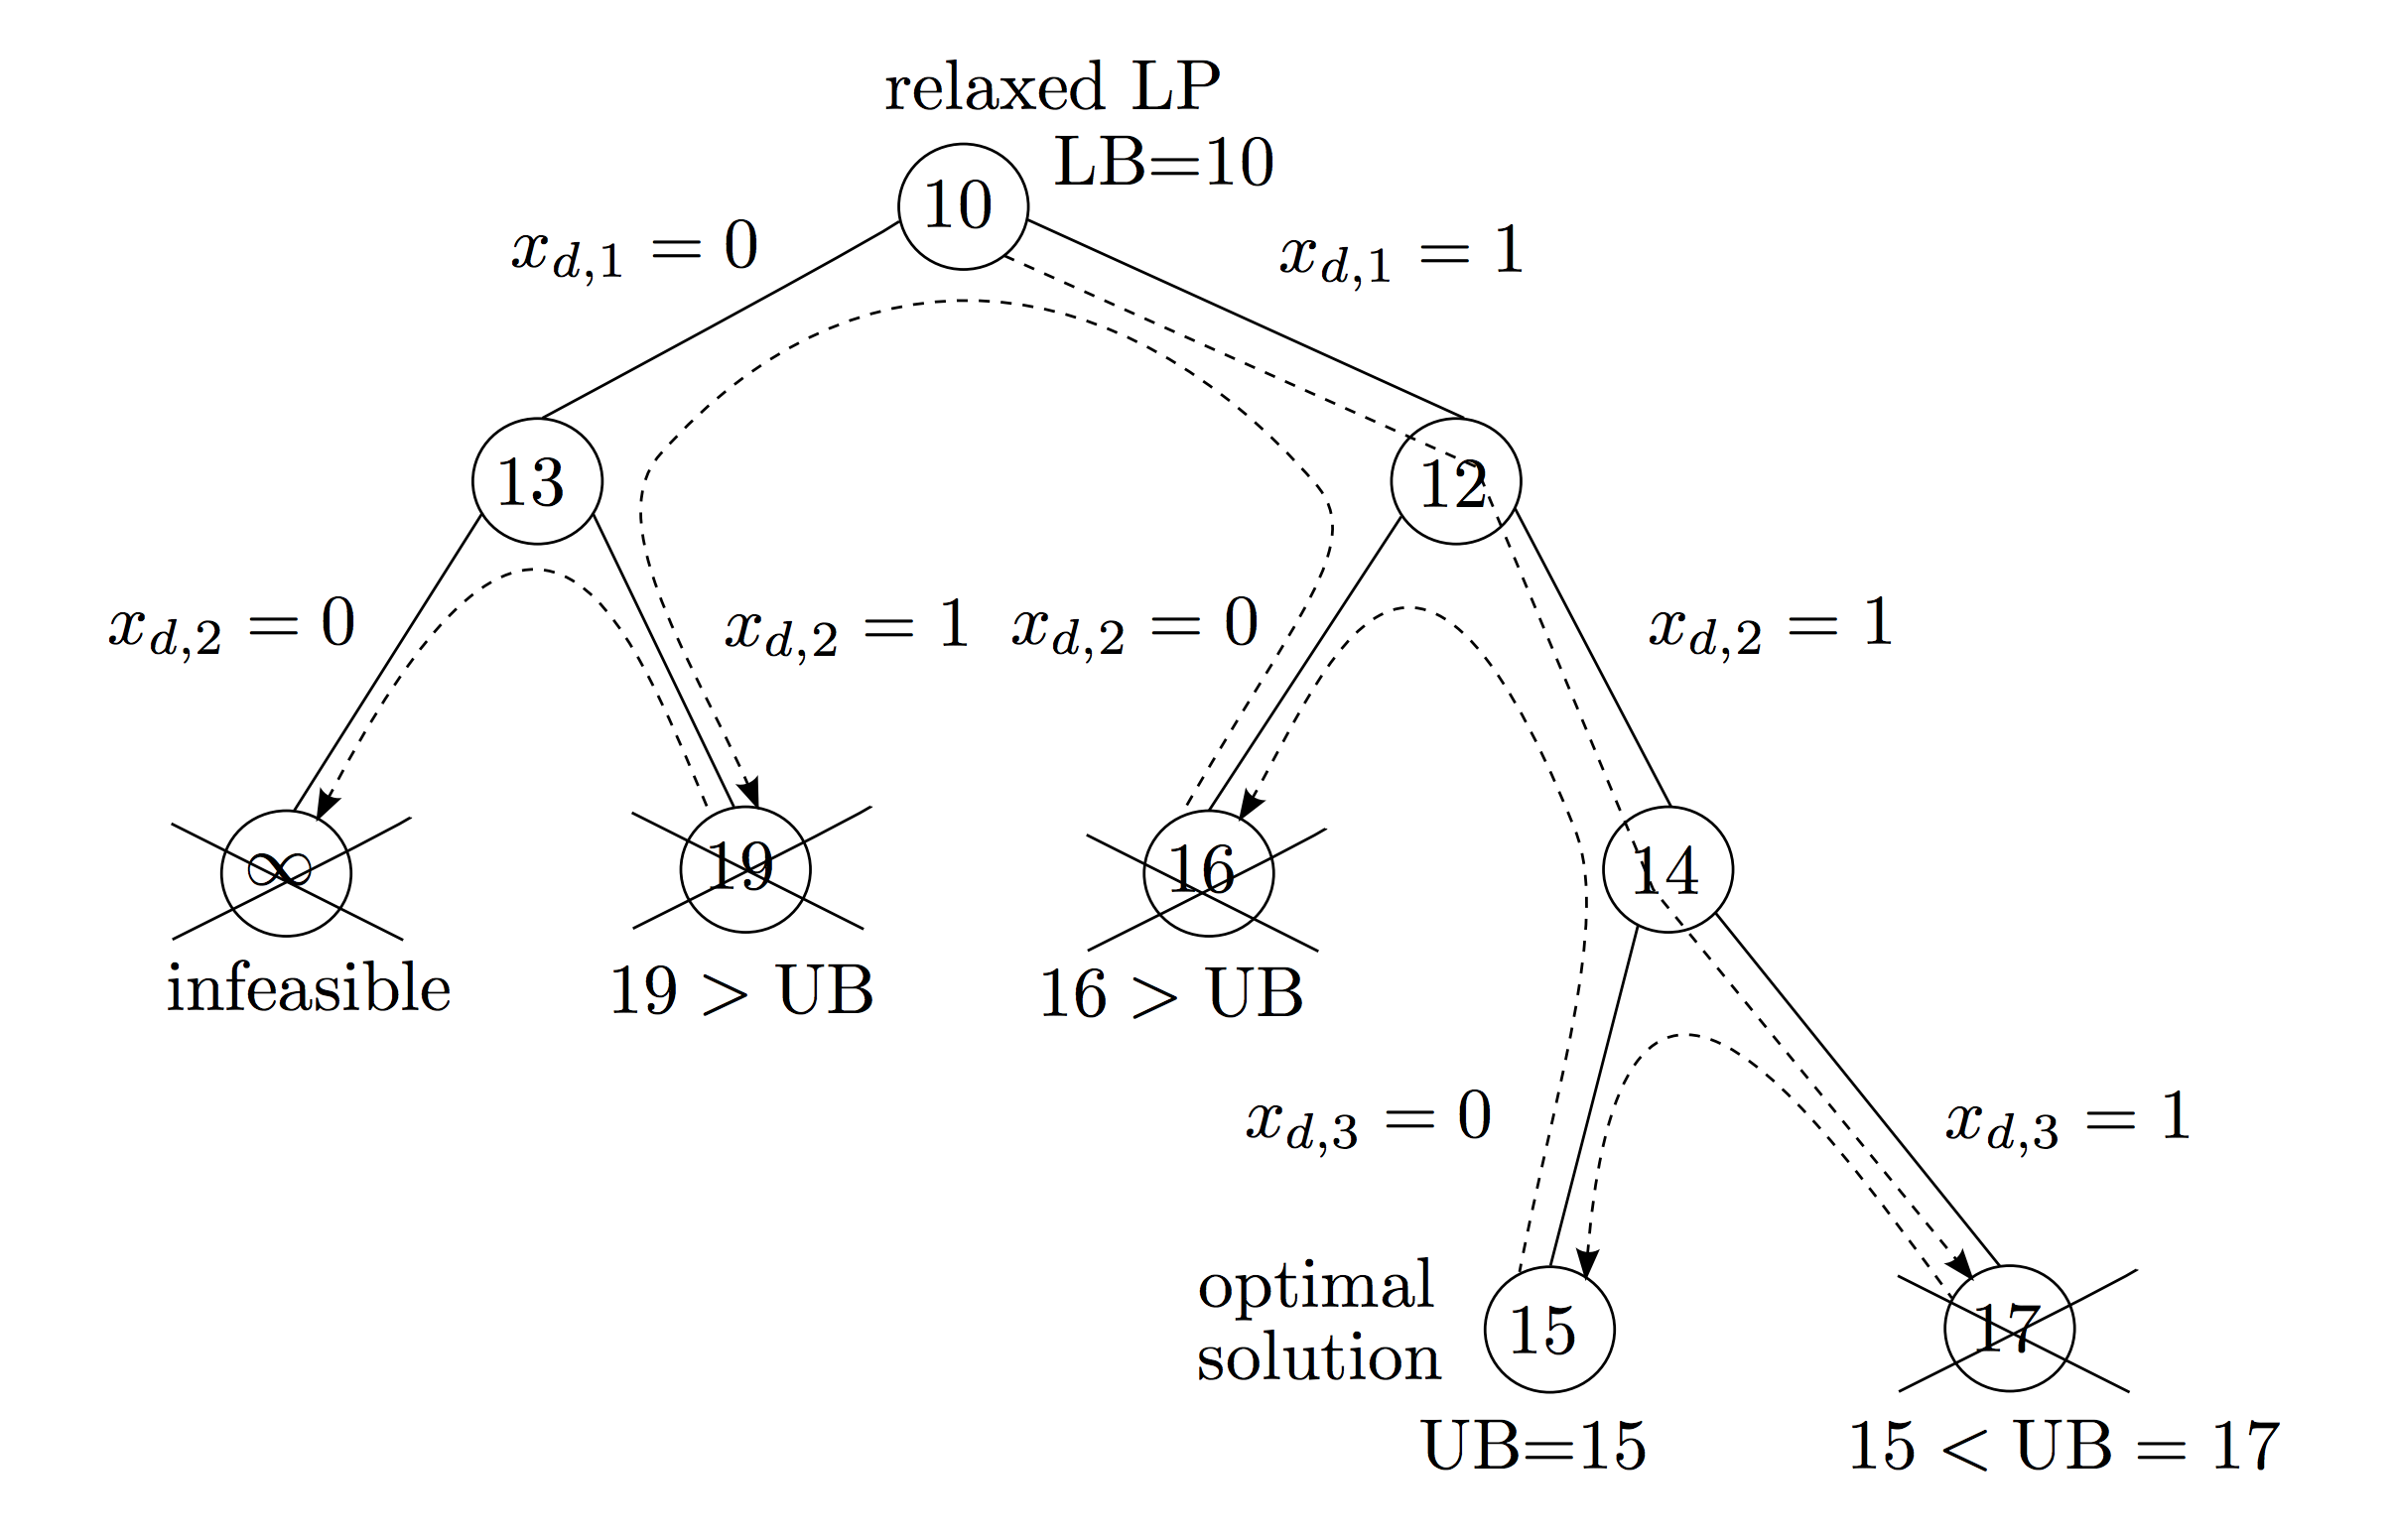
\includegraphics[scale=0.2]{bnb.png}
\section{Numerical Optimization -- Iterative Methods}
\subsection{Gradient descent}
$x_{i+1} = x_i \remph{-} h_i\nabla f(x_i)$ with step-size $h_i = \dfrac{1}{L}$ for
$L$-smooth $f(x)$:
\begin{align*}
\exists L: \lVert \nabla f(x) &- \nabla f(y) \rVert \leq L \lVert x - y \rVert \; \forall x, y, \in \R^n \\
\iff & \nabla f \text{ is Lipschitz continuous} \\
\iff & f \text{ can be upperbounded by a quadratic function: } \\
f(x) \le f(y) + &\nabla f(y)^T(x - y)+ 0.5L\left\| x-y\right\|^2 \forall x, y \in\R^n
\end{align*}

\subsection{Newton's Method}
\begin{align*}
x_{i+1} = x_i \remph{+} h_i\Delta x_{nt} := x_i \remph{-} h_i (\nabla^2 f(x_i))^{-1} \nabla f(x_i)
\end{align*}
Line search problem: choose $h_i > 0$ s.t. $f(x_i + h_i\Delta x_{nt}) \leq f(x_i)$. \\
Either compute exact and best $h_i$ using:
\begin{align*}
h_i^* = \text{argmin } x_i + h_i\Delta x_{nt}
\end{align*}

Or use the backtracking search method:
\begin{align*}
&\text{For } \alpha \in (0, 0.5) \text{ and } \beta \in (0,1): \\
&	\quad \text{Initialise } h_i = 1; \\
&	\quad \text{while } f(x_i+ h_i\Delta x_{nt}) > f(x_i) + \alpha h_i \nabla f(x_i)^T\Delta x_{nt} \text{ do } h_i \leftarrow \beta h_i
\end{align*}

For given equality constraint $\vA x = b$ solve:
\begin{align*}
\Me{\nabla^2 f(x_i) & \vA^T \\ \vA & \bm 0}\Me{\Delta x \\ \lambda} = \Me{-\nabla f(x_i) \\ \bm 0}
\end{align*}

\subsection{Constrained optimization with $g_i(x) \leq 0$}
\paragraph{Gradient method}
$x_{i+1} = \pi_Q(x_i - h_i\nabla f(x_i))$ where $\pi_Q$ is a projection $\pi_q = \arg\min_x\frac{1}{2}\lVert x - y \rVert_2^2$. Projection can be solved directly if simple enough, else solve the dual.

\subsection{Interior-Point methods}
Assumptions $f(x^*) < \infty$, $\tilde x \in \dom(f)$.

\paragraph{Barrier method}
$\min f(x) + \kappa \phi(x)$.
Approximate $\phi$ using diff'able log barrier(instead of indicator function):
\begin{align*}
\phi(x) &= \sum_{i=1}^{m} I\_(g_i(x)) = -\sum_{i=1}^{m} \log(-g_i(x)) \\
        & \lim_{\kappa \rightarrow 0} x^*(\kappa) = x^*
\end{align*}
Analytic center: $\arg\min_x \phi(x)$, central path $\left\{x^*(\kappa) \middle| \kappa > 0 \right\}$.

\paragraph{Path following method} \ \newline
1. Centering 
$x^*(\kappa) = \arg\min_x f(x) + \kappa\phi(x)$ with newton's method: \\
1.1. $\Delta x_\text{nt} = \left[\nabla^2 f(x) + \kappa \nabla^2\phi(x)\right]^{-1}(-\nabla f(x) - \kappa \nabla \phi(x))$. \\
1.2. Line search:
\begin{align*}
\text{retain feasability: } & \argmax_{h > 0} \left\{ h \middle| g_i(x+h\Delta x) < 0 \right\} \\
\text{Find } h^* = & \argmin_{h\in[0,h_\text{max}]} \left\{ f(x+h\Delta x) + \kappa\phi(x+h\Delta x) \right\}
\end{align*}
2. Update step $x_i = x^*(\kappa_i)$ \\
3. Stop if $m\kappa_i \leq \epsilon$ \\
4. Decrease $\kappa_{i+1} = \kappa_{i}/\mu$, $\mu > 1$.

\paragraph{Centering step with equality constraints}
\begin{align*}
\Me{\nabla^2 f(x) + \kappa \nabla^2\phi(x) & c^T \\ c & \bm 0} \Me{\Delta x_\text{nt} \\ \nu} & = -\Me{\nabla f(x) + \kappa\nabla\phi(x) \\ 0}
\end{align*}

\paragraph{Relaxed KKT}
\begin{align*}
Cx^* & = d & g_i(x^*) + s_i^* & = 0 \\
\nabla f(x^*) + \sum_{i=1}^{m} \lambda_i^*\nabla g_i(x^*) + c^T \nu & = 0 & \lambda_i^* = \kappa\frac{\partial\phi}{\partial g_i} & = -\frac{\kappa}{g_i} \\
\lambda_i^*g_i(x^*) & = - \kappa & \lambda_i^*, s_i^* & \geq 0
\end{align*}

\paragraph{Primal Dual Search Direction Computation}
\begin{align*}
\Me{H(x,\lambda) & c^T & G(x)^T & 0 \\ c & 0 & 0 & 0 \\ G(x) & 0 & 0 & \vI \\ 0 & 0 & \vS & \bm \Lambda}\Me{\Delta x \\ \Delta u \\ \Delta \lambda \\ \Delta s} & = - \Me{\nabla f(x) + c^T\nu + G(x)^T\lambda \\ cx - d \\ g(x) + s \\ s\lambda - \nu}
\end{align*}
$\vS = \diag(s_1, \dots, s_m), \bm \Lambda = \diag(\lambda_1, \dots, \lambda_m)$ and \\
$\nu$ is a vector for choosing centering parameters.


\end{multicols*}

\end{document}
